\chapter{Reducing the computational cost}
\label{ch:reducing}

\begin{itemize}
	\item As mentioned in section , evaluating the objective function needs
computing all the pairwise distances between the points. Also, the evaluating
the gradient is expensive. This is done in $\mathcal{O}(N^2D^2)$ flops. So it is
not trivial to successfully use NCA on large data sets.
	\item This chapter presents a wide palette of ideas and methods that can be
applied to speed up the computations. Most of the methods rely on the fact that
the learnt metric is low ranked.
	\item Every method presented can be regarded as an alteration of the original
objective function. We basically change our objective function such that the new
objective will have a reduced cost.
\end{itemize}

\section{Sub-sampling}
\label{sec:sub-sampling}

Sub-sampling is the simplest idea that can help speeding up the computations.
For the training procedure we use a randomly selected sub-set $\mathcal{D}_n$ of
the original data set $\mathcal{D}$:
 \[
 	\mathcal{D}_n = \{ \xB_{i_1},\cdots,\xB_{i_n} \} \subseteq \mathcal{D}.
 \]
 If $n$ is the size of the sub-set then the cost of the gradient is reduced to
$\mathcal{O}(n^2D^2)$. After the projection matrix $\AB$ is learnt, it can be
applied to the whole data set and all the data points are used for
classification.

While easy to implement, this method discards a lot of information available.
Also it is affected by the fact the sub-sampled data has a thinner distribution
than the real data. 

\begin{figure}
  \centering
  \subfigure[Learnt projection $\AB$ on the sub-sampled data set
$\mathcal{D}_n$.]{\label{fig:sub-sampling-1}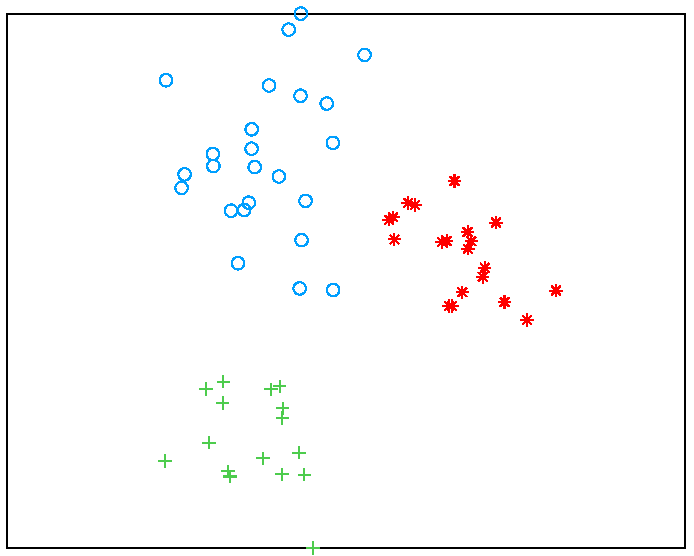
\includegraphics[width=0.48\textwidth]{images/sub-sample-1}}
\subfigure[The projection $\AB$ applied to the whole data set
$\mathcal{D}$.]{\label{fig:sub-sampling-2}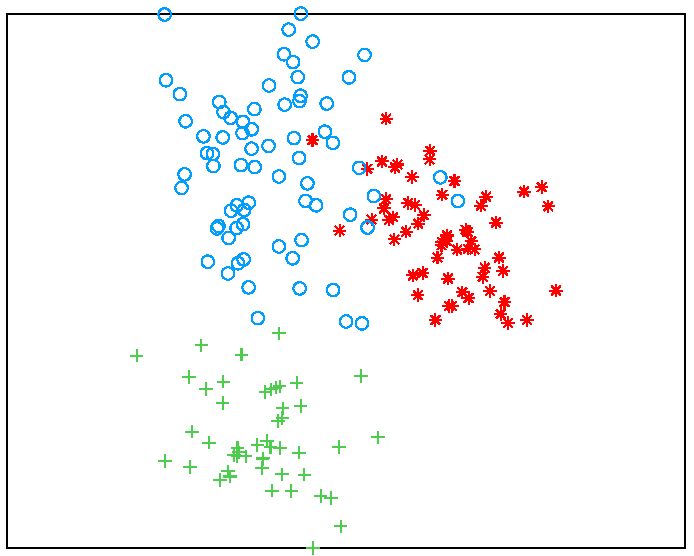
\includegraphics[width=0.48\textwidth]{images/sub-sample-2}}
  \caption{Result of sub-sampling method on \texttt{wine}. There were used one
third of the original data set for training, \textit{i.e.}, $n = N/3$. We note
that the points that belong to the sub-set $\mathcal{D}_n$ are perfectly
separated. But after applying the metric to the whole data there appear
different misclassifications. The effects are even more acute if we use smaller
sub-sets.}
  \label{fig:sub-sampling}
\end{figure}

\section{Mini-batches}
\label{sec:mini-batches}

The next obvious idea is to use sub-sets in an iterative manner, similar to the
stochastic gradient descent method: split the data into mini-batches and train
on them successively. Again the cost for one evaluation of the gradient will be
$\mathcal{O}(n^2D^2)$ if the mini-batch consists of $n$ points.

\begin{algorithm} 
	\caption{Training algorithm using mini-batches formed by clustering} 
	\label{alg:mini-batches}  
	\begin{algorithmic} [1]                 % enter the algorithmic environment
		\REQUIRE Data set $\mathcal{D}=\{\xB_1,\cdots,\xB_N\}$ and initial linear
transformation $\AB$.
		\REPEAT
			\STATE Project each data point using $\AB$: 
$\mathcal{D}_\AB=\{\AB\xB_1,\cdots,\AB\xB_N\}$.
			\STATE Use either algorithm \ref{alg:fpc} or \ref{alg:rpc} on
$\mathcal{D}_\AB$ to split $\mathcal{D}$  into $K$ mini-batches
$\mathcal{M}_1,\cdots,\mathcal{M}_K$.
			\FORALL {$\mathcal{M}_i$}
				\STATE {Update parameter: $\AB\leftarrow \AB - \eta\frac{\partial
f(\AB,\mathcal{M}_i)}{\partial\AB}$.}
				\STATE {Update learning rate $\eta$.}
			\ENDFOR
		\UNTIL {convergence.}
	\end{algorithmic}
\end{algorithm}

There are different possibilities for splitting the data-set:
\begin{enumerate}
	\item Random selection. In this case the points are assigned randomly to each
mini-batch and after one pass through the whole data set another random
allocation is done. As in section \ref{sec:sub-sampling}, this suffers from the
thin distribution problem. In order to alleviate this and achieve convergence,
large-sized mini-batches should be used (similar to Laurens van der Maaten's
implementation). The algorithm is similar to Algorithm \ref{alg:mini-batches},
but lines 2 and 3 will be replaced with a simple random selection.
	
	\item Clustering. Constructing mini-batches by clustering ensures that the
point density in each mini-batch is conserved. In order to maintain a low
computational cost, we consider cheap clustering methods, \textit{e.g.},
farthest point clustering (FPC; \citealp{gonzalez1985}) and recursive projection
clustering (RPC; \citealp{chalupka2011}). Algorithm 
	
	FPC gradually selects cluster centres until it reaches the desired number of
clusters $K$. The point which is the farthest away from all the current centres
is selected as new centre. The precise algorithm is presented below.
	
	\begin{algorithm} 
		\caption{Farthest point clustering} 
		\label{alg:fpc}  
		\begin{algorithmic}                    % enter the algorithmic environment
			\REQUIRE Data set $\mathcal{D}=\{\xB_1,\cdots,\xB_N\}$ and $K$ number of
clusters.
			\STATE Randomly pick a point that will be the first centre $\cB_1$.
			\STATE Allocate all the points in the first cluster $\mathcal{M}_1 \leftarrow
\mathcal{D}$.
			\FOR {$i=1$ to $K$}
				\STATE Select the $i$-th cluster centre $\cB_i$ as the point that is
farthest away from any cluster centre $\cB_1,\cdots,\cB_{i-1}$.
				\STATE Move to the cluster $\mathcal{M}_i$ those points that are closer to
its centre than to any other cluster centre: $\mathcal{M}_i = \left\{ \xB \in
\mathcal{D} \;| \; d(\xB;\cB_i) < d(\xB;\cB_j), \forall j \neq i \right\}$
			\ENDFOR
		\end{algorithmic}
	\end{algorithm}
	
	This computational cost of this method is $\mathcal{O}(NK)$. However, we do not
have any control on the number of points in each cluster, so we might end up
with very unbalanced clusters. A very uneven split has a couple of obvious
drawbacks: too large mini-batches will maintain high cost, while on too small
clusters there is not too much too learn.
	
	So, as an alternative, RPC was especially developed to mitigate this problem.
It constructs the clusters similarly to how the $k$-d trees are build (see
section ). However instead of splitting the data set across axis aligned
direction it chooses the splitting directions randomly (see algorithm
\ref{alg:rpc}). So, because it uses the median value it will result in similar
sized clusters and we can easily control the dimension of each cluster. The
complexity of this algorithm is $\mathcal{O}()$.
	
	\begin{algorithm} 
		\caption{Recursive projection clustering} 
		\label{alg:rpc}  
		\begin{algorithmic}                    % enter the algorithmic environment
			\REQUIRE Data set $\mathcal{D}=\{\xB_1,\cdots,\xB_N\}$ and $n$ size of
clusters.
			\IF {$N < n$}
				\STATE New cluster: $i\leftarrow i+1$.
				\RETURN current points as a cluster: $\mathcal{M}_i \leftarrow \mathcal{D}$.
			\ELSE
				\STATE {Randomly select two points $\xB_j$ and $\xB_k$ from $\mathcal{D}$.}
				\STATE {Project all data points onto the line defined by $\xB_j$ and
$\xB_k$. (Give equation?)}
				\STATE {Select the median value $\tilde{\xB}$ from the projected points.}
				\STATE {Recurse on the data points above and below $\tilde{\xB}$:
$\text{RPC}(\mathcal{D}_{>\tilde{\xB}})$ and
$\text{RPC}(\mathcal{D}_{\le\tilde{\xB}})$.}
%							$\mathcal{D}_{>\tilde{\xB}}=\{\xB\in\mathcal{D}|\xB>\tilde{\xB}\}$
			\ENDIF
		\end{algorithmic}
	\end{algorithm}
	
	Note that we are re-clustering in the transformed space after one sweep through
the whole data set. There are also other alternatives. For example, we could
cluster in the original space periodically or we could cluster only once in the
original space. However the proposed variant has the advantage of a good
behaviour for a low rank projection matrix $\AB$. Not only that is cheaper, but
the clusters resulted in low dimensions by using RPC are closer to the real
clusters then applying the same method in a high dimensional space. 
	
	Further notes:
	\begin{itemize}
		\item The learning rate can be updated using various heuristics as presented
in the section related to optimization.
		\item The convergence can be tested in various ways: stop when there is not
enough momentum in the parameter space, when the function value doesn't vary too
much or by using early stopping or a maximum number of iterations. Discuss all
of these in practical issues section.
	\end{itemize}
	
\end{enumerate}

%\begin{center}
%	\begin{table}
%		\centering
%		\begin{tabular}{l}
%			\toprule
%			Training algorithm using mini-batches\\
%			\midrule
%			\textbf{Do}\\
%			Split data $\mathcal{D}$ into mini-batches:
%$\mathcal{M}_1,\cdots,\mathcal{M}_m$,\\
%			such that $\mathcal{M}_1\cup\cdots\cup\mathcal{M}_m=\mathcal{D}$\\
%			\textbf{For each} mini-batch $\mathcal{M}_i$\\
%			$\AB\leftarrow \AB - \eta\frac{\partial
%f(\AB,\mathcal{M}_i)}{\partial\AB}$\\
%			\textbf{End for}\\
%			\textbf{Until} we reach convergence\\
%			\bottomrule
%		\end{tabular}
%		\caption{Algorithm for training with mini-batches. The learning is done using
%gradeint ascent.}
%	\end{table}
%\end{center}


\section{Stochastic learning}
\label{sec:stochastic-learning}

The following technique is theoretically justified by stochastic approximation
arguments. The main idea is to get an unbiased estimator of the gradient by
looking only at a few points and how they relate to the entire data set.

More precisely, in the classical learning setting, we update our parameter $\AB$
after we have considered each point $\xB_i$ in the data set. In the stochastic
learning procedure, we update $\AB$ more frequently by considering only $n$
randomly selected points. As in the previous case, we still need to compute
$\{p_i\}_{i=1}^n$ using all the $N$ points. It should be further stressed the
difference to the mini-batches approach; there, the contributions are calculated
only between the $n$ points that belong to the mini-batch. 

The objective function that we need to optimize at each iteration and its
gradient are given by the next equations:
\begin{align}
	f_\text{sNCA}(\AB) = \sum_{i=1}^n p_i\\
	\frac{\partial f_\text{sNCA}}{\partial \AB} = \sum_{i=1}^{n} \frac{\partial
p_i}{\partial \AB}
	\label{eq:snca-grad}
\end{align}
This means that the theoretical cost of the stochastic learning method will
scale with $nN$.

	\begin{algorithm} 
		\caption{Stochastic learning for NCA (sNCA)} 
		\label{alg:sNCA}  
		\begin{algorithmic}                    
			\REQUIRE Data set $\mathcal{D}=\{\xB_1,\cdots,\xB_N\}$, $n$ number of points
to consider for the gradient estimation, $\AB$ initial linear transformation.
			\REPEAT
				\STATE Split data $\mathcal{D}$ into groups $\mathcal{M}_i$ of size $n$.\
				\FORALL {$\mathcal{M}_i$}
					\STATE {Update parameter using gradient given by Equation
\ref{eq:snca-grad}: \STATE $\AB\leftarrow \AB - \eta\frac{\partial
f_\text{sNCA}(\AB,\mathcal{M}_i)}{\partial\AB}$.}
					\STATE {Update learning rate $\eta$.}
				\ENDFOR
			\UNTIL {convergence.}
		\end{algorithmic}
	\end{algorithm}

Note: this idea might be used easily and robustly for on-line learning. Given a
new point $\xB_{N+1}$ we update $\AB$ using the derivative $\frac{\partial
p_{N+1}}{\partial \AB}$.

\section{Approximate computations}
\label{sec:approximate}

A straightforward way of speeding up the computations was previously mentioned
in the original paper \citep{goldberger2004} and in some NCA related work
\citep{weinberger2007, singh2010}. The observations involve pruning small terms in
the original objective function. We then use an approximated objective function
and its corresponding gradient for the optimization process.

\begin{figure}
	\centering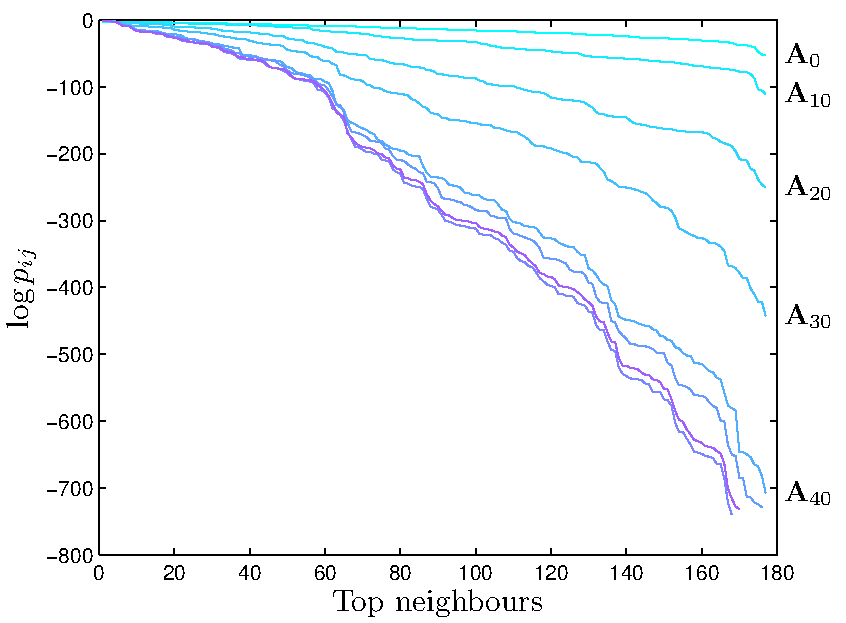
\includegraphics[width=0.7\textwidth]{images/contributions}
	\caption{Evolution of the stochastic assignments $p_{ij}$ during training for a given point $\xB_i$.}
	\label{fig:contributions}
\end{figure}

The motivation lies in the fact that the contributions $p_{ij}$ decay very
quickly with distance:
 \[
 	p_{ij} \propto \exp\{-d(\AB\xB_i;\AB\xB_j)^2\}.
 \] 
 
 The evolution of the contributions during the training period is depicted in
Figure \ref{fig:contributions}.  We notice that most of the values $p_{ij}$ are insignificant compared
to the largest contribution. This suggests that we might be able to preserve the
accuracy of our estimations even if we discard a large part of the neighbours.

So, \citet{weinberger2007} choose to use only the top $m = 1000$ neighbours for
each point $\xB_i$. Also they disregard those points that are farther away than
$d_{\max}=34$ units from the query point: $p_{ij} = 0, \forall \xB_j$ such that
$d(\AB\xB_i;\AB\xB_j)>d_{\max}$. While useful in practical situations, these
suggestions lack of a principled description: how can we optimally choose $m$
and $d_{\max}$ in a general setting? We would also like to be able to estimate
the error introduced by the approximations.

We correct those drawbacks by making use of the KDE formulation of NCA (see
Section \ref{sec:cc-kde}) and adapting existing ideas for fast KDE
\citep{deng1995,gray2003} to our particular application. We will use a class of
accelerated methods that are based on data partitioning structures
(\textit{e.g.}, $k$-d trees, ball trees). As we shall shortly see, these provide
us with means to quickly find only the neighbours $\xB_j$ that give significant
values $p_{ij}$ for any query point $\xB_i$. 
%Hence, we will be able to compute an approximated value of the true
%class-conditional probability $p(\xB_i|c) = \sum_{j\in c}
%k(\xB_i|\xB_j),\forall i,c.$
%
%A question still remains: given a point $\xB_i$ how can we \textit{quickly} ?
%It is clear that only the nearby points will contribute to $p_i$, while the
%points that are further away can be ignored. A framework that provides us with
%means of doing this is the $k$-d tree.

\subsection{$k$-d trees}
\label{subsec:k-d-trees}

The $k$ dimensional tree structure ($k$-d tree; \citealp{bentley1975}) organises
the data in a binary tree using axis-aligned splitting planes. The $k$-d tree
has the property to place close in the tree those points that live nearby in the
original geometrical space. This makes such structures efficient mechanisms for
nearest neighbour searches \citep{friedman1977} or range searches
\citep{moore1991}.

There are different flavours of $k$-d trees. We choose for our application a
variant of $k$-d tree that uses bounding boxes to describe the position of the
points. Intuitively, we can imagine each node of the tree as a bounding
hyper-rectangle in the $D$ dimensional space of our data. The root node will
represent the whole data set and it can be viewed as an hyper-rectangle that
contains all the data points, see Figure \ref{fig:kdtree-1}. In the two-dimensional presented exampled, the points are enclosed by rectangles. From Figure \ref{fig:kdtree-1} to \ref{fig:kdtree-4}, there are presented the existing bounding boxes at different levels of the binary tree. To understand how these are obtained, we discuss the $k$-d tree construction.

\begin{figure}
  \centering
  \subfigure[Root
node]{\label{fig:kdtree-1}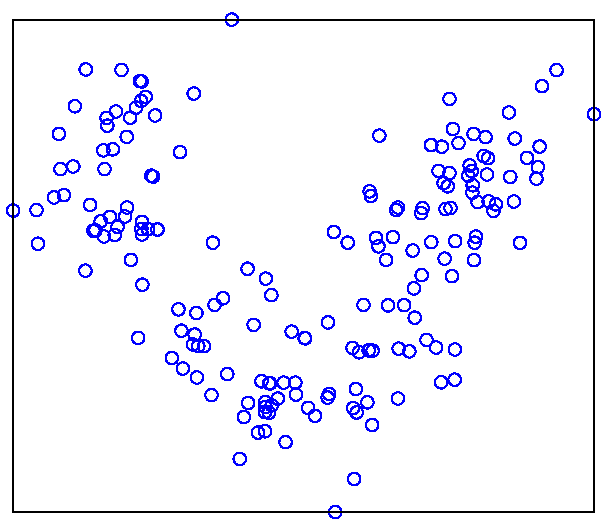
\includegraphics[width=0.45\textwidth]{images/kdtree-1}}
\subfigure[First
level]{\label{fig:kdtree-2}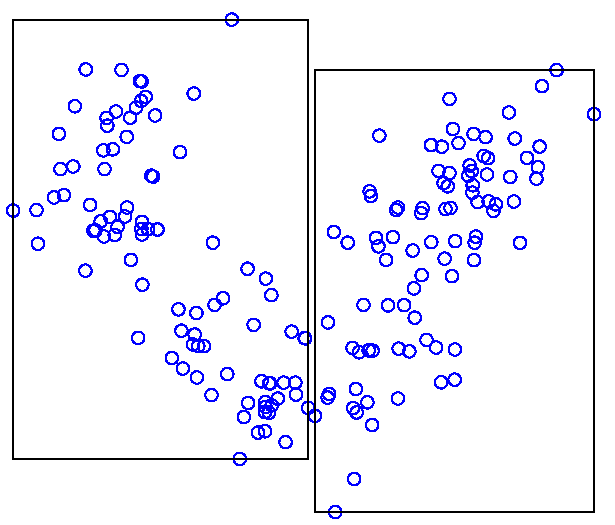
\includegraphics[width=0.45\textwidth]{images/kdtree-2}}
\\
  \subfigure[Second
level]{\label{fig:kdtree-3}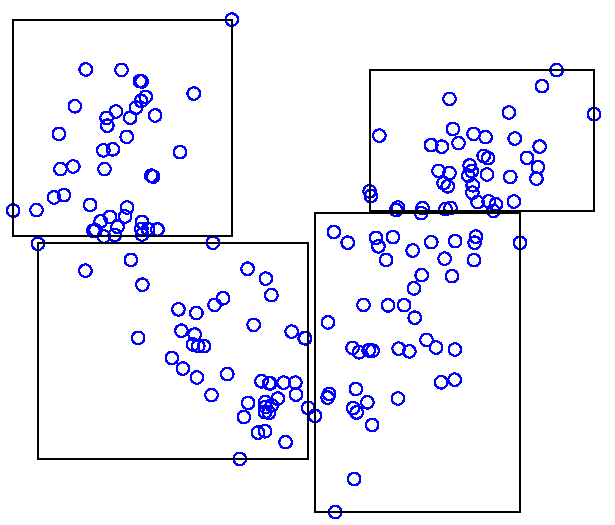
\includegraphics[width=0.45\textwidth]{images/kdtree-3}}
\subfigure[Last
level]{\label{fig:kdtree-4}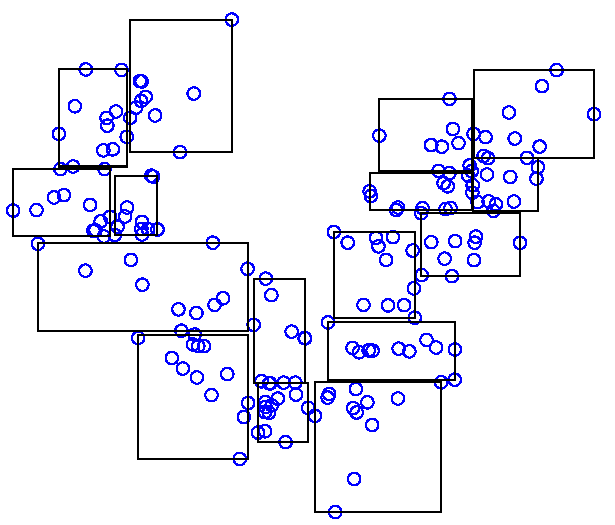
\includegraphics[width=0.45\textwidth]{images/kdtree-4}}
  \caption{Illustration of the $k$-d tree with bounding boxes at different
levels of depths. This figure also outlines the building phases of the tree.}
  \label{fig:kdtree}
\end{figure}

The building of the tree starts from the root node and is done recursively. At each
node we select which of the points from the current node will be allocated to each of
the two children. Because these are also described by hyper-rectangles, we just have to select a splitting plane. Then the two successors will consist of the points from the two sides of the hyper-plane. 

A splitting hyper-plane can be fully defined by two parameters: a direction $\vec{d}$ on which the plane is perpendicular and a point $P$  that is in the plane. Given that the splits are axis aligned, there are $D$ possible directions $\vec{d}$. We can either choose this randomly or we can use
each of the directions from $1$ to $D$ in a successive manner. A more common approach is to choose $\vec{d}$ to be the dimension that presents the largest
variance: 
\begin{align}
	\vec{d} \leftarrow \operatorname{argmax}_{d} (\max_ix_{id} -
\min_ix_{id}).
	\label{eq:splitting-direction}
\end{align}

This results in a better clustering of the points and the shape of the bounding boxes will be closer to the shape of a square. Otherwise it might happen that points situated in the same node can still be further away.

Regarding the splitting value $P$, a usual choice is the median value $\tilde{x}_d$ on the previously selected direction $\vec{d}$. This choice of $P$ guarantees a balanced tree which offers several advantages. We can allocate static memory for the entire data structure. This is faster to access than dynamical allocation. Also a balanced tree has a better worst case complexity than an unbalanced one. Other useful implementation tricks that can be applied to balanced $k$-d trees are suggested by \cite{lang2009}.

After the splitting plane is chosen, the left child will contain the points that are on the left of the hyper-plane: 
\begin{align}
\mathcal{D}_{\le \tilde{x}_d} = \{ \xB \in \mathcal{D}_{\xB_i}| x_{d} \le \tilde{x}_d \},
\label{eq:subset-left}
\end{align}
 where $\mathcal{D}_{\xB_i}$ denotes the data points bounded by the current node $\xB_i$. Similarly, the right child will contain the points that are placed on the right of the hyper-plane:
\begin{align}
\mathcal{D}_{> \tilde{x}_d} = \{ \xB \in \mathcal{D}_{\xB_i}| x_{d} > \tilde{x}_d \}.
\label{eq:subset-right}
\end{align}

This process is repeated until the number of points bounded by the current node goes below a threshold $m$. These nodes are the leaves of the tree and they store the effective points. The other non-leaf nodes store information regarding the bounding box and the splitting plane. Note that a hyper-rectangle is completely defined by only two $D$-dimensional points, one for the ``top-right'' corner and the other for the ``bottom-left'' corner. 

	\begin{algorithm} 
		\caption{$k$-d tree building algorithm} 
		\label{alg:kd-tree-build}  
		\begin{algorithmic}                    % enter the algorithmic environment
			\REQUIRE Data set $\mathcal{D}=\{\xB_1,\cdots,\xB_N\}$, $i$ position in tree
and $m$ number of points in leaves.
			\IF {$N < m$}
				\STATE Mark node $i$ as leaf: \texttt{splitting\_direction(i)=-1}.
				\STATE Add points to leaf: \texttt{points(i)}$\leftarrow \mathcal{D}$.
				\RETURN
			\ENDIF
				\STATE {Choose direction $\vec{d}$ using Equation
\ref{eq:splitting-direction}:}
				\STATE {\texttt{splitting\_direction(i)=}$d$.}
				\STATE {Find the median value $\tilde{x}_d$ on the direction $\vec{d}$:}
				\STATE {\texttt{splitting\_value(i)=}$\tilde{x}_d$.}
				\STATE {Determine the subsets of points that are separated by the resulting splitting plane: $\mathcal{D}_{\le\tilde{\xB}}$ and $\mathcal{D}_{>\tilde{\xB}}$, see Equations \ref{eq:subset-left} and \ref{eq:subset-right}.}
				\STATE {Build left child
\texttt{build\_kdtree(}$\mathcal{D}_{\le\tilde{\xB}}$\texttt{,2*i)}.}
				\STATE {Build right child
\texttt{build\_kdtree(}$\mathcal{D}_{>\tilde{\xB}}$\texttt{,2*i+1)}.}
%							$\mathcal{D}_{>\tilde{\xB}}=\{\xB\in\mathcal{D}|\xB>\tilde{\xB}\}$
		\end{algorithmic}
	\end{algorithm}
	
 	The most used operation on a $k$-d tree is the nearest neighbour (NN) search. While we will not apply pure NN for the next method, we will use similar concepts. However, we can do NN retrieval with $k$-d trees after we applied NCA, as suggested by \citet{goldberger2004}. The search in the $k$-d tree is done in a depth-first search manner: start from the root and traverse the whole tree by selecting the closest node to the query point. In the leaf, we find the nearest neighbour from the $m$ points and store it and the corresponding distance $d_\text{min}$. Then we recurs up the tree and look at the farther node. If this is situated at a minimum distance that is smaller than $d_\text{min}$, we have to investigate also that node. In the other case, we can ignore the node and all the points it contains. Usually, a large fraction of the points can be omitted, especially when the data has structure.
 	It is important to stress that the performance of $k$-d trees quickly degrades with the number of dimensions the data lives. 
 	
 	%Hence, it is useful to understand how the search is done and how computational saving are achieved. 
	
%	\begin{itemize}
%		\item 
%		\item So we will be able to efficiently use $k$-d trees only when learning a
%low-rank $\AB$ that projects the data points in a low dimensional space.
%	\end{itemize}
	
%organize the data in a binary tree structure using axis-aligned splitting
%planes of the data space. Each node in the tree represents a data point and it
%also contains a splitting direction (this is usually denoted by an integer from
%1 to $k$). The splitting plane is often chosen to be perpendicular on the
%dimension with the largest variance and to go through the median point (this
%results in a balanced tree). Furthermore, a non-leaf node has two successors:
%the sub-tree rooted at the left successor contains the points that are situated
%at the left of the splitting plane, while the sub-tree rooted at the right
%successor of the splitting plane contains the points that are situated at the
%right of the splitting plane. 

\subsection{Approximate kernel density estimation}
\label{subsec:approx-kde}

\begin{itemize}
	\item The following ideas are mostly inspired by previous work on fast kernel
density estimators \citep{gray2003,shen2006}.
	\item The goal is to compute $p(\xB)$. In the kernel density estimation, we
estimate the unknown probability density function as follows: $p(\xB_i) =
\frac{1}{N}\sum_{j=1} Nk(\xB_i|\xB_j)$. If the number of samples $N$ is large
then $p(\xB_i)$ can approximated to high degree of precision by discarding lots
of the data. A question still remains: how can we do this in a sensible manner? 
	\item Given a query point $\xB$ and a group of points $G$ we can replace each
individual contribution $k(\xB|\xB_j), \xB_j\in G$, with $k(\xB|\xB_g)$. This
last quantity is specific for the group and will be common for all points in
$G$. There are two ways to obtain a reasonable value for $k(\xB|\xB_g)$: either
approximate $\xB_g$ first and then compute $k(\xB|\xB_g)$; here $\xB_g$ can be
the mean of the points in the group. The second possibility is to approximate
$k(\xB|\xB_g)$ directly; one possibility is $k(\xB|\xB_g) =
\frac{\min_jk(\xB|\xB_j) + \max_jk(\xB|\xB_j)}{2}$. We prefer the second option,
because it does not need to store mean of the points from $G$. Also, we will see
that the minimum and maximum contributions have to be computed to decide whether
to prune or not; so no further computational expense is introduced by using this
approximation.
	\item We can see that the maximum error for each point in the group that is
introduced by such an approximation is $\frac{\max_jk(\xB|\xB_j) -
\min_jk(\xB|\xB_j)}{2}$. This can be controlled to be small; for example, we can
decide to approximate only when the group is far away from the query point or
when the kernel contribution is almost constant for the points within the group.
However, it is better to consider the error relative to the total quantity we
want to estimate. But we do not know the total sum before hand so we will use an
upper bound $p(\xB) < p_{\text{SoFar}}(\xB) + \max k(\xB|\xB_j) $. This means
that the order in which we accumulate it is important. 
	\item By using $k$-d trees our groups will be hyper-rectangles. So in order to
prune we test that the largest and the smallest contribution within the
hyper-rectangle varies a little. We start at with a large group, the root of the
tree, that contains all the points and then recurs on its children until there
is no need to and we can approximate. 
\end{itemize}

\subsection{Approximate KDE for NCA}
\label{subsec:approx-KDE-for-NCA}
	\begin{itemize}
		\item NCA was formulated as a class-conditional kernel density estimation
problem. So we evaluate $p(\xB|c),\forall c$ and for each class we build a $k$-d
tree. We will obtain an approximated version of the objective function. To
obtain the gradient of this new objective function we can use Equation
\ref{eq:nca-cc-kde-grad}. The derivative of $p(\AB\xB|c)$ will be different only
for those groups where we do approximations. So, for such a group we obtain the
following gradient:
		\begin{align}
			\frac{\partial}{\partial \AB} \sum_{j\in G} k(\AB\xB|\AB\xB_j) &\approx
\frac{\partial}{\partial \AB} \frac{1}{2} \left\{\min_{j\in G}
k(\AB\xB|\AB\xB_j) + \max_{j\in G} k(\AB\xB|\AB\xB_j)\right\}\notag\\
			& = \frac{1}{2}\left\{ \frac{\partial}{\partial \AB} k(\AB\xB|\AB\xB_c) +
\frac{\partial}{\partial \AB} k(\AB\xB|\AB\xB_f) \right\},
		\end{align}
		where $\AB\xB_c$ denotes the closest point in $G$ to the query point $\AB\xB$
and $\AB\xB_f$ is the farthest point in $G$ to $\AB\xB$. Here we made use of the
fact the kernel function is a monotonic function of the distance. So the closest
point gives the maximum contribution, while the farthest point contributes the
least.
	\end{itemize}
	
	
	\begin{algorithm} 
		\caption{Approximate NCA objective function and gradient computation} 
		\label{alg:cc-kde-nca}  
		\begin{algorithmic}                    % enter the algorithmic environment
			\REQUIRE Projection matrix $\AB$, data set
$\mathcal{D}=\{\xB_1,\cdots,\xB_N\}$ and error~$\epsilon$.
			\FORALL {classes $c$}
				\STATE {Build $k$-d tree for the points in class $c$.}
			\ENDFOR 
			\FORALL {data points $\xB_i$}
				\FORALL {classes $c$}
					\STATE {Compute estimated probability $\hat{p}(\AB\xB_i|c)$ and the
corresponding derivatives $\frac{\partial}{\partial \AB} \hat{p}(\AB\xB_i|c)$ 
using approximated KDE Algorithm:}
%					\STATE {\texttt{[p(c),dp(c)]=NCA\_recursive(kdtree(c))}}
				\ENDFOR
				\STATE Compute soft probability $\hat{p}_i \equiv \hat{p}(c|\AB\xB_i) =
\frac{\hat{p}(\AB\xB_i|c_i)}{\sum_{c}\hat{p}(\AB\xB_i|c)}$.
				\STATE Compute gradient $\frac{\partial}{\partial \AB} \hat{p}$ using
Equation \ref{eq:nca-cc-kde-grad}.
				\STATE Update function value and gradient value.
			\ENDFOR
		\end{algorithmic}
	\end{algorithm}
	
	
	
\section{Exact computations}
\label{sec:exact-computations}

	Exact methods are the counterpart of approximate methods. We can have both efficient and exact computations just by modifying the NCA model. Again, the idea is motivated by the rapid decay of the
	exponential function. Instead of operating on very small values, we will make them exactly zero. This is achieved by replacing the squared exponential kernel with a compact support function. So, the points that lie outside the support of the kernel are ignored and just a fraction of the total number of points is used for computing the contributions $p_{ij}$. Further gains in speed are obtained if the search for those points is done with $k$-d trees (the range search algorithm is suitable for this task; \citealp{moore1991}).
	
	The choice of the compact support kernel is restricted by a single requirement: differentiability. We will use the simplest polynomial function that has this property. This is given by the
	following expression:
	\begin{align}
		k_{\text{CS}}(u)=\begin{cases}
			c\;(a^2-u^2)^2& \mbox{if } u \in [-a;+a]\\
			0& \mbox{otherwise},\\
		\end{cases}
		\label{eq:cs-1}
	\end{align}
	where $c$ is a constant that controls the height of the kernel and $a$ is a constant that controls the width of the kernel. In the given context, the kernel will be a function of the distance between two points: $k_{\text{CS}}(u)=k_{\text{CS}}(d_{ij})$, where $d_{ij} = d(\AB\xB_i;\AB\xB_j)$. Note that the constant $a$ can be absorbed by the linear projection $\AB$. This means that the scale of the learnt metric will compensate for the kernel's width. Also the value for $c$ is not important: from Equation \ref{eq:stochastic-neighbours-cs} we see that this reduces. For convenience, we set both $a=1$ and $c=1$. So, we obtain the following simplified version of the kernel:
	\begin{align}
		k_{\text{CS}}(d_{ij})= (1-d_{ij}^2)^2\;\mathrm{I}(\left|d_{ij}\right|\le1),
	\end{align}
	where $\mathrm{I}(\cdot)$ denotes the indicator function: $\mathrm{I}(\cdot)$ return 1 when its argument is
	true and 0 when its argument is false.
	
	Now we reiterate the steps of the NCA algorithm (presented in Section \ref{sec:general-presentation}), and replace $\exp(\cdot)$ with $k_\text{CS}(\cdot)$. We obtain the following new stochastic neighbour assignments:
	\begin{align}
		q_{ij} = \frac{k_{\text{CS}}(d_{ij})}{\sum_{k\neq i} k_{\text{CS}}(d_{ik})}.
		\label{eq:stochastic-neighbours-cs}
	\end{align}
	
	These can be compared to the classical soft assignments given by Equation \ref{eq:stochastic-neighbour}. Next we do not need to change the general form of the objective function: 
	\begin{align}
		f_\text{CS}(\AB) = \sum_{i}\sum_{j\in c_i} q_{ij}.
	\end{align}
	
	In order to derive the gradient of the function $f_\text{CS}$, we start by computing the gradient of the kernel:
	\begin{align}
		\frac{\partial}{\partial\AB}k_\text{CS}(d_{ij}) 
		&= 
	\frac{\partial}{\partial\AB}\left[(1-d_{ij}^2)^2\cdot\mathrm{I}(\left|d_{ij}\right|\le
	1)\right]\notag\\
		&= -4\AB(1-d_{ij}^2)  \xB_{ij} \xB_{ij}^\mathrm{T} \cdot
	\mathrm{I}(\left|d_{ij}\right|\le 1),\label{eq:nca-cs-grad-kernel}
	\end{align}
	where $\xB_{ij}=\xB_i-\xB_j$.
	
	The gradient of the new objective function is:
	\begin{align}
		\frac{\partial f_\text{CS}}{\partial \AB}=4\AB\sum_{i=1}^{N}
		\left(
		q_i \sum_{k=1}^N \frac{q_{ik}}{1-d_{ik}^2} \xB_{ik}\xB_{ik}^{\textrm{T}}
		- \sum_{j\in c_i} \frac{q_{ij}}{1-d_{ij}^2}\xB_{ij}\xB_{ij}^{\textrm{T}} 
		\right).
		\label{eq:nca-cs-grad}
	\end{align}
	
	This method can be applied in same way as classic NCA: learn a metric $\AB$ that maximizes the objective function $f_\text{CS}(\AB)$. Since the function is differentiable, any gradient based method is suitable for optimization and can be used on Equation \ref{eq:nca-cs-grad}.
	
	There is one concern with the compact support version of NCA. There are situations when a point $\xB_i$ is placed outside the support of any other point in the data set. Intuitively, this means that the point $\xB_i$ is not selected by any point, hence it is not assigned any class label. Also this causes mathematical problems: as in Subsection \ref{subsec:numerical-issues}, the contributions $p_{ij}$ will have an indeterminate value $\frac{0}{0}$. Except of the log-sum-exp trick, the advice from Subsection \ref{subsec:numerical-issues} can be applied here as well. A more robust way of dealing with this is discussed in the next Section.
	
%	The main concern with this method is what happens when points lie outside the
%	compact support of any other point in the data set. So care must be taken at
%	initialisation. One way would be to initialise with a very small scale $\AB$.
%	However, this means that there is no gain in speed for at least the first
%	iterations. It might be better to use the principal components for
%	initialisation. 
	
\section{NCA with compact support kernels and background distribution}
\label{sec:nca-cs-back}

	\begin{figure}
	  \centering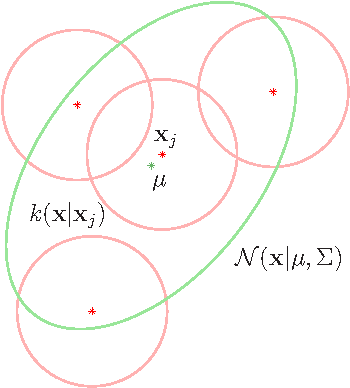
\includegraphics[width=6cm]{images/nca-cs-back}
	  \caption{Neighbourhood component analysis with compact support kernels and
	background distribution. The main assumption is that each class is a mixture of
	compact support distributions $k(\xB|\xB_j)$ plus a normal background
	distribution $\mathcal{N}(\xB|\muB,\SigmaB)$.}
	  \label{fig:cs-back}
	\end{figure}
	
	We extend the previous model to handle cases where points fall outside the support of any other neighbours. The idea is to use  for each class a background distribution that explains the unallocated points. The background distribution should have an infinite support and an obvious example is the normal distribution.
	
	To introduce a background distribution in a principled manner, we return to the class conditional kernel density estimation (CC-KDE) formulation of NCA, Section \ref{sec:cc-kde}. First, we recast the compact support NCA in the probabilistic framework and consider each class as mixture of compact support distributions: 
	\begin{align}
		p(\xB_i|c) = \frac{1}{N}\sum_{j\in c} k_\text{CS}(\xB_i|\xB_j),
	\end{align}
	where $k_\text{CS}(\xB_i|\xB_j) = k_\text{CS}(d_{ij})$ and is defined by Equation \ref{eq:cs-1}. Because $k_\text{CS}(\xB_i|\xB_j)$ denotes a distribution, it ought to integrate to 1. For $c=\frac{15}{16}$ and $a=1$ the requirement is satisfied.
	
	We further change the model and incorporate an additional distribution in the class-conditional probability $p(\xB_i|c)$. From a generative perspective this can be interpreted as follows: a point $\xB_i$ is generated by either the compact support distribution from each point $k_\text{CS}(\xB_i|\xB_j)$ or by a class-specific normal distribution $\mathcal{N}(\xB_i|\muB_c,\SigmaB_c)$. So, the distribution $p(\xB_i|c)$ can be written as the sum of these components:
		\begin{align}
			p(\xB_i|c) = \beta \mathcal{N}(\xB_i|\muB_c,\SigmaB_c) + (1-\beta)
	\frac{1}{N_c}\sum_{j\in c} k_\text{CS}(\xB_i|\xB_j),
			\label{eq:nca-cs-back-1}
		\end{align}
	where $\beta$ is the mixing coefficient between the background distribution and
	the compact support model, $\muB_c$ is the sample mean of the class $c$ and $\SigmaB_c$ is the sample
	covariance of the class $c$. The constant $\beta$ can be set to $\frac{1}{N_c+1}$. This will give equal weights to the background distribution and to each compact support distribution. It might be better to treat $\beta$ as a parameter and fit it during training. We expect $\beta$ to adapt to the data set: for example, $\beta$ should increase for data sets with convex classes. 
	
	To finalize this method, we just need to plug Equation \ref{eq:nca-cs-back-1} into
	the set of Equations \ref{eq:nca-cc-kde-bayes}, \ref{eq:nca-cc-kde-obj} and
	\ref{eq:nca-cc-kde-grad}. The only difficulty is the gradient computation. We give here only derivatives for each individual component (the full derivations and equations can be found in the Appendix):
	\begin{itemize}
%		\item $\beta = \frac{1}{N_c+1}$ we will give equal weights to the background
%	distribution as to the compact-support distribution. Setting it too large means
%	that the model will favour convex classes. On one hand, this might diminish
%	NCA's power. One of its strengths lies in the ability to work on non-convex
%	classes. On the other hand, some of the classes  This can be fitted as a
%	parameter during the optimization process. The gradient with respect to $\beta$
%	can be easily derived and it is easy to evaluate it as the quantities required
%	for this should also be computed for the function evaluation. 
		\item The gradient of the compact support distribution $k_\text{CS}(\xB_i|\xB_j)$ with respect to $\AB$ is very similar to what is given in Equation \ref{eq:nca-cs-grad-kernel}. The only difference is that in this case we have everything multiplied by the constant $c=\frac{15}{16}$.
		\item For the gradient of the background distribution it is useful to note that projecting the points $\{\xB_i\}_{i=1}^N$
	into a new space $\{\AB\xB_i\}_{i=1}^N$ will change the sample mean $\muB_c$ to
	$\AB\muB_c$ and the sample covariance $\SigmaB_c$ to
	$\AB\SigmaB_c\AB^\mathrm{T}$. Hence, we have:
		\begin{align}
			\frac{\partial}{\partial \AB} \mathcal{N}(\AB\xB_i&|\AB\muB_c, \AB\SigmaB_c
	\AB^\mathrm{T}) = \mathcal{N}(\AB\xB_i|\AB\muB_c, \AB\SigmaB_c
	\AB^\mathrm{T})\notag\\
			&\times \{ -(\AB\SigmaB_c \AB^\mathrm{T})^{-1}\AB\SigmaB_c
			+\vB \vB ^ \mathrm{T} \AB \SigmaB_c - \vB (\xB - \muB_c)^\mathrm{T}
			\},
		\end{align}
		where $\vB = (\AB\SigmaB_c \AB^\mathrm{T})^{-1}\AB(\xB - \muB_c)$.
		\item If we also consider $\beta$ a parameter, we also need the derivative of the objective function with respect to $\beta$. This can be easily obtained, if we use the derivative of the class conditional distribution with respect to $\beta$:
		\begin{align}
			\frac{\partial}{\partial\beta} p(\xB_i|c) 
			=  \mathcal{N}(\xB_i|\muB_c,\SigmaB_c) -
				\frac{1}{N_c}\sum_{j\in c} k_\text{CS}(\xB_i|\xB_j).
		\end{align}
		
	\end{itemize}

